\chapter{Adaptation d'un maillage de surface dynamique}

\textit{Objectif du chapitre: on veut mettre au point une méthodologie pour déformer un maillage de l'interface en propagation en utilisant le modèle \brep\ dynamique comme support géométrique, afin de pouvoir réaliser des simulations EF/VF dans des domaines de géométrie déformable.}

\par\bigskip

Motivation
\begin{enumerate}
	\item les méthodes (EF, VF, \ldots) employées pour la simulation numérique nécessitent un \textit{maillage} du (volume du) domaine de calcul
	\item la précision et la vitesse de convergence du calcul dépendent fortement de la qualité (forme et taille) des éléments du maillage
\end{enumerate}

\section{Problématique et état de l'art}

\subsection{Simulation numérique dans un domaine à géométrie déformable}
\begin{enumerate}
	\item maillage volumique (fluide) conforme à l'interface
	\begin{enumerate}
		\item \label{item:methodo_bodyfitted_ALE} 1 seul maillage \anglais{body-fitted} avec formulation ALE \emph{(ref)}
		\begin{itemize}
			\item principe : frontière = maillage de l'interface, intérieur déformé de façon arbitraire (purement lagrangien si la vitesse de déformation du maillage est imposée par le champ de vitesse du fluide)
			\item intérêt/avantages : \ldots
			\item contraintes/inconvénients : 
			\begin{itemize}
				\item la qualité du maillage volumique dépend fortement de celle du maillage surfacique, surtout dans les régions proches de l'interface, où ont généralement lieu les phénomènes physiques les plus pertinents
				\item la connectivité du maillage doit rester fixe \emph{(à vérifier)}
			\end{itemize}
		\end{itemize}
		
		\item plusieurs maillages \anglais{body-fitted} qui se superposent
		\begin{itemize}
			\item méthode Chimère \cite{meakin1989, wang2000}, FLUSEPA \cite{brenner1991}
			\item intérêt/avantages : 
			\begin{itemize}
				\item facilite la génération du maillage volumique lorsque la géométrie est complexe (\eg hyper-sustentateurs)
				\item évite de déformer un maillage 3d
			\end{itemize}						
			\item contraintes/inconvénients : 
			\begin{itemize}
				\item nécessite de traiter les intersections entre les blocs de maillage
				\item limité aux mouvements rigides \emph{(à vérifier)}
			\end{itemize}
		\end{itemize}
	\end{enumerate}
	
	\item maillage volumique non-conforme à l’interface
	\begin{itemize}
		\item méthode des frontières immergées \cite{peskin2002, hovnanian2012, wang2012} : interface représentée explicitement, volume (fluide) traité de façon eulérienne (\ie maillage fixe)
		\item intérêt/avantages : évite de générer et déformer un maillage 3d autour d’une géométrie complexe
		\item contraintes/inconvénients : application indirecte des conditions aux limites
	\end{itemize}
\end{enumerate}

Dans cette thèse,
\begin{enumerate}
	\item on ne traite que le maillage (surfacique) de l'interface
	\item on se concentre sur des maillages triangulaires linéaires par morceaux, mais une extension aux maillages hybrides et courbes (high-order) est envisageable
\end{enumerate}






\subsection{Génération de maillage surfacique basé sur un modèle \brep}
Essentiellement extension de méthodes standard (\ie quadtree, Delaunay, avancée de front) 2d plan à des surfaces immergées/plongées dans $\reals^3$
\begin{enumerate}
	\item méthodes indirectes (Riemanniennes) : on travaille dans l'espace paramétrique en tenant compte de la métrique (anisotrope, Riemannienne) induite par la paramétrisation de façon à ce que le plongement du maillage dans $\reals^3$ respecte les critères prescrits
	\begin{enumerate}
		\item conforme à la topologie \brep\ : on exploite directement les paramétrisations locales (carreaux de surface) du modèle \brep\ \cite{borouchaki2000} (on maille d'abord les sommets, puis les arêtes et enfin les faces afin de garantir la conformité du maillage)
		\begin{itemize}
			\item intérêt/avantages : utilisation de méthodes 2d plan robustes et efficaces
			\item contraintes/inconvénients : les arêtes \brep\ douces introduisent des contraintes supplémentaires sur le maillage, sans avoir de signification du point du vue du calcul EF/VF $\Rightarrow$ éléments de mauvaise qualité
		\end{itemize}
		\item trans-carreaux par (re-)paramétrisation globale : l'idée générale est de construire une transformation affine par morceaux (par triangles) l'espace $uv$ de chacune des faces qui composent une nappe et un l'espace $uv$ global de cette nappe, sans affecter la définition géométrique du modèle \brep\ sous-jacent
			\begin{enumerate}
			
				\item \cite{marcum1999} :
				\begin{enumerate}
					\item on construit d'abord un maillage de référence conforme à la topologie \brep\ d'un ensemble de faces regroupées
					\item \label{item:bouche_trous} on bouche artificiellement les éventuels \guillemets{trous} afin qu'il n'y ait qu'un seul bord
					\item on plonge ce maillage dans un espace paramétrique global :
					\begin{itemize}
						\item afin d'obtenir les coordonnées paramétriques globales des n\oe uds intérieurs, on résout un système d'équations elliptique (opérateur Laplacien combinatoire) avec une condition de Dirichlet pour fixer les n\oe uds du bord sur un cercle
						\item on modifie les coordonnées paramétriques globales des n\oe uds du bord afin d'améliorer la forme des éléments incidents
						\item (on répète le processus jusqu'à ce que la qualité des éléments dans l'espace paramétrique global soit convenable)
					\end{itemize}
					\item on élimine les éventuels éléments fictifs créés à l'étape \ref{item:bouche_trous}
					\item on génère une triangulation dans l'espace paramétrique global par avancée de front en utilisant le maillage de référence comme approximation géométrique dans l'espace physique
					\item on retrouve les coordonnées paramétriques locales des n\oe uds du nouveau maillage 
					\item limites : la nappe doit avoir au moins un bord
				\end{enumerate}
				
				\item \cite{noel2002} : 
				\begin{enumerate}
					\item le domaine paramétrique de chaque face \brep\ est décomposé en cellules triangulaires s'appuyant sur les contours
					\item chaque cellule (courbe) est en bijection avec un triangle (linéaire) dans l'espace paramétrique global de la nappe
					\item une triangulation du domaine paramétrique global (convexe) est générée (quadtree-Delaunay) 
					\item limites : la nappe doit avoir au moins un bord
				\end{enumerate}
				
				\item \cite{jones2004} :
				\begin{enumerate}
					\item on part ici aussi d'une triangulation de référence conforme à la topologie \brep\ (\ie chaque face a sa propre triangulation)
					\item l'assemblage des faces en nappes est réalisé directement dans le plan $(u,v)$ à partir des plongements de leur triangulation respective dans leur espace paramétrique local
					\item une face de ``base'' est choisie, le plongement de sa triangulation dans l'espace paramétrique global est identique à celui dans son espace paramétrique local
					\item les triangulations des faces adjacentes sont ensuite plongées une à une dans l'espace $uv$ global à l'aide d'une technique d'avancée de front qui préserve la forme des triangles
					\item limites : 
					\begin{itemize}
						\item cette approche peut échouer si les plongements des triangulations de deux faces adjacentes dans leur espace $uv$ respectif ont des rapports d'échelles différents au niveau d'une arête commune %suivant les deux directions paramétriques
						\item il semblerait que les nappes doivent ici aussi avoir au moins un bord
					\end{itemize}
					
				\end{enumerate}
			\end{enumerate}
		\begin{itemize}
			\item intérêt/avantages : lève les contraintes topologiques du modèle \brep\ qui ne sont pas pertinentes pour le calcul EF/VF, sans en affecter la définition géométrique
			\item limites/inconvénients : 
			\begin{itemize}
				\item topologie : limité aux nappes avec un ou plusieurs bords $\Rightarrow$ nécessite un découpage (généralement manuel) de l'interface
				\item géométrie : limité aux nappes quasi-planes et régulières
			\end{itemize}
			
		\end{itemize}
	\end{enumerate}
	
	\item méthodes directes : 
	\begin{enumerate}
		\item \cite{lau1996} : avancée de front directement dans $\reals^3$ avec projection sur la surface exacte des n\oe uds au cours de la génération $\to$ limité à une paramétrisation continue (\ie carreau par carreau, conforme à la topologie \brep)
		\item \cite{foucault2013} : avancée de front directe trans-carreaux
	\end{enumerate}
\end{enumerate}







\subsection{Optimisation de maillage surfacique}
\begin{figure}
\centering
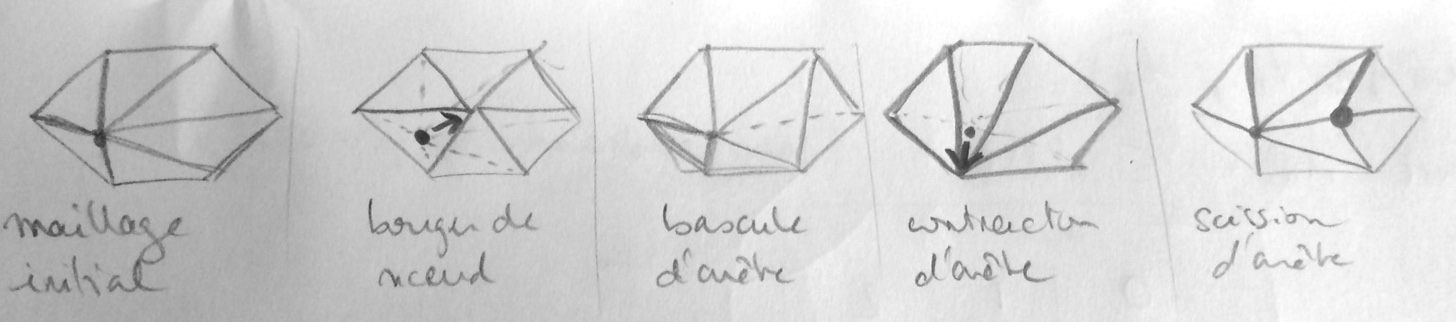
\includegraphics[width=\textwidth]{operations_locales_optimisation_maillage}
\caption{\ldots}
\label{fig:operations_locales_optimisation_maillage}
\end{figure}

\begin{enumerate}
	\item bouger de n\oe ud (direct, \ie $xyz$ ou indirect, \ie $uv$)
	\begin{enumerate}
		\item méthodes heuristiques (lissage laplacien, analogies physiques \cite{farhat1998}, interpolation (IDW, RBF, \ldots) \ldots)
		\item lissage basé sur l'optimisation d'une métrique de qualité \cite{freitag1995, canann1998, jiao2008} \cite{gargallo2014} $\to$ maillage supporté sur un carreau de surface paramétrique
	\end{enumerate}
	\item changements locaux de connectivité
	\begin{enumerate}
		\item bascule d'arête
		\item contraction d'arête
		\item scission d'arête
	\end{enumerate}
\end{enumerate}

%Dans cette thèse,
%\begin{enumerate}
%	\item (\autoref{item:methodo_bodyfitted_ALE})/de nombreux codes de calculs ne tolèrent pas les changement de connectivité en cours de calcul $\Rightarrow$ on se concentre essentiellement sur le bouger de n\oe ud (déformation pure) 
%	\item on n'effectuera des reconnections locales qu'en dernier recours (remaillage)
%\end{enumerate}



\par\bigskip
le maillage doit être une approximation géométrique fidèle de l’interface (dont la géométrie
« exacte » est définie par le modèle \brep)\\
$\to$ solution la plus simple : le maillage interpole la surface \brep\ aux n\oe uds (qui sont alors localisés sur des entités \brep\ et donc sur un ou plusieurs carreaux de surface) $\Rightarrow$ l'écart de corde doit être contrôlé (taille d'élément dicté par le rayon de courbure local, maillage explicite des caractéristiques/singularités géométriques (arêtes vives, coins, \ldots))


\section{Lien entre modèle \brep\ et maillage trans-carreaux}
Objectifs :
\begin{enumerate}
	\item \label{item:limiter_ecart_corde} représenter fidèlement la surface (courbe) à l'aide d'un maillage (linéaire) (\ie limiter/contrôler l'écart de corde)
	\item \label{item:alleger_contraintes_topo} s'affranchir au maximum des contraintes sur le maillage inutilement imposées par la topologie du modèle \brep\ (arêtes douces)
\end{enumerate}

Essentiellement, on veut que le maillage respecte la \textit{géométrie} du modèle \brep, mais pas nécessairement sa \textit{topologie}.

\subsection{Construction d'une structure d'hypergraphe}


\section{Déformation de maillage trans-carreaux basé sur un modèle \brep\ dynamique}
Objectifs :
\begin{enumerate}
	\item \label{item:preserver_connect} préserver autant que faire se peut la connectivité du maillage (éviter de générer un nouveau maillage à chaque pas de temps)
\end{enumerate}

\subsection{Correspondance d'hypergraphes}


\subsection{Régénération du maillage contraint}

\subsection{\anglais{Untanglement}}

\subsection{Optimisation par bouger de n\oe ud}
\label{section:projection_surface_composite}
Décrire la procédure de projection d'un déplacement sur la surface \brep\ (sur une hyper-face ou une hyper-arête)
$\rightarrow$ trajectoire trans-carreaux \cite[Section~5.5]{foucault2008}), \cite{thompson2005}, \cite[p.42 et Section~4.4.1]{crozet2017}

\subsection{Optimisation par reconnections locales}
\subsubsection{Bascule d'arête}
Les arêtes contenues dans les chaînes ne peuvent pas être basculées.

\subsubsection{Contraction d'arête}
Soit $e$ l'arête entre les n\oe uds $p_1$ et $p_2$. Sans restreindre la généralité, on supposera que $\ddl(p_1) \leq 
\ddl(p_2)$.
Ici, $\ddl(p)$ représente le nombre de degrés de liberté du n\oe ud $n$, \ie 
\begin{itemize}
	\item $\ddl(p) = 0$ si $n$ est contraint sur un sommet \brep\ ;
	\item $\ddl(p) = 1$ si $n$ est contraint sur une hyper-arête (chaîne) ;
	\item $\ddl(p) = 2$ si $n$ n'est pas contraint (ou plutôt est contraint sur une hyper-face).
\end{itemize}
Si $\ddl(p_1) = \ddl(p_2) = 1$, la contraction n'est possible que si $e$ fait partie d'une chaîne, \ie les n\oe uds $p_1$ et $p_2$ sont contraints sur la même hyper-arête (voir \autoref{fig:contraction_arete_cas_1_1}).

\setlength{\imagewidth}{50mm}
\begin{figure}
  \centering
  %
  \hspace*{\fill}
  \subbottom[L'arête $e_2$ peut être contractée, mais pas $e_1$ puisque ses extrémités sont contenues dans deux chaînes distinctes (en rouge et vert).]{
	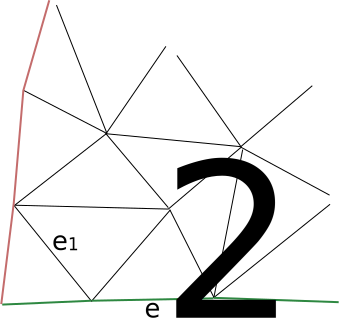
\includegraphics[width=\imagewidth]{contraction_arete_cas_1_1_avant}
	\label{fig:contraction_arete_cas_1_1_avant}
  }
  \hfill%
  \subbottom[Maillage résultant de la contraction de l'arête $e_2$.]{
	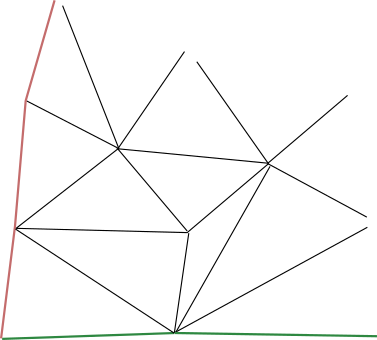
\includegraphics[width=\imagewidth]{contraction_arete_cas_1_1_apres}
	\label{fig:contraction_arete_cas_1_1_apres}
  }
  \hspace*{\fill}
  \caption{Deux cas possibles pour une arête dont les deux sommets ont un seul degré de liberté.}
  \label{fig:contraction_arete_cas_1_1}
  %
\end{figure}

Si $\ddl(p_1) < \ddl(p_2)$ on contracte $e$ vers le n\oe ud $p_1$. 
Si $\ddl(p_1) = \ddl(p_2)$ on contracte $e$ vers son milieu. Afin de localiser précisément ce milieu sur la surface \brep\ (\ie connaître l'entité \brep\ qui le supporte, ainsi que ses coordonnées paramétriques dans les carreaux de surface concernés), on calcule la projection sur la surface \brep\ du n\oe ud $p_1$ translaté d'un vecteur $\frac{p_2 - p_1}{2}$ (voir \autoref{fig:contraction_arete_milieu}), en suivant la procédure décrite dans la \autoref{section:projection_surface_composite}.

\setlength{\imagewidth}{50mm}
\begin{figure}
  \centering
  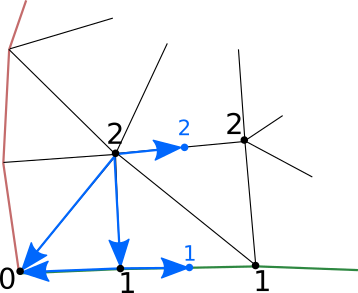
\includegraphics[width=\imagewidth]{contraction_arete_milieu}
  \caption{Placement du n\oe ud résultant de la contraction d'une arête. Le $\ddl$ de chaque n\oe ud concerné est indiqué à côté de celui-ci. Les flèches représentent les vecteurs déplacement à projeter pour chaque arête contractée.}
  \label{fig:contraction_arete_milieu}
\end{figure}


\subsubsection{Scission d'arête}
On insère un n\oe ud au milieu d'une arête. Comme pour la contraction d'arête, les coordonnées de ce milieu sont une nouvelle fois obtenue par la procédure de projection décrite dans la \autoref{section:projection_surface_composite}.
Cette fois, la projection du déplacement se fait en partant du sommet de l'arête ayant le plus grand nombre de degrés de liberté, comme illustré sur la \autoref{fig:scission_arete_milieu}.

\setlength{\imagewidth}{50mm}
\begin{figure}
  \centering
  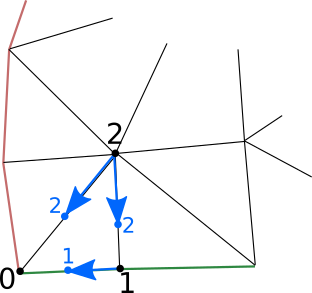
\includegraphics[width=\imagewidth]{scission_arete_milieu}
  \caption{Placement du nouveau n\oe ud résultant d'une scission d'arête. Le $\ddl$ de chaque n\oe ud concerné est indiqué à côté de celui-ci. Les flèches représentent les vecteurs déplacement à projeter pour chaque arête scindée.}
  \label{fig:scission_arete_milieu}
\end{figure}



